\section{離散フーリエ変換}

音声や電流といった信号を計測したとき,それらの値は時間領域における電気信号の連続データ(アナログデータ)
として出力される.
連続データはコンピュータ上で扱うことができないので,連続データを
ある一定間隔でサンプリングすることでコンピュータ上で扱える離散データ(デジタルデータ)
へ変換することでコンピュータ上でのデータの取得,解析が可能となる(\autoref{fig:digital_sin}).
\iffigure
\begin{figure}[h]
  \centering
  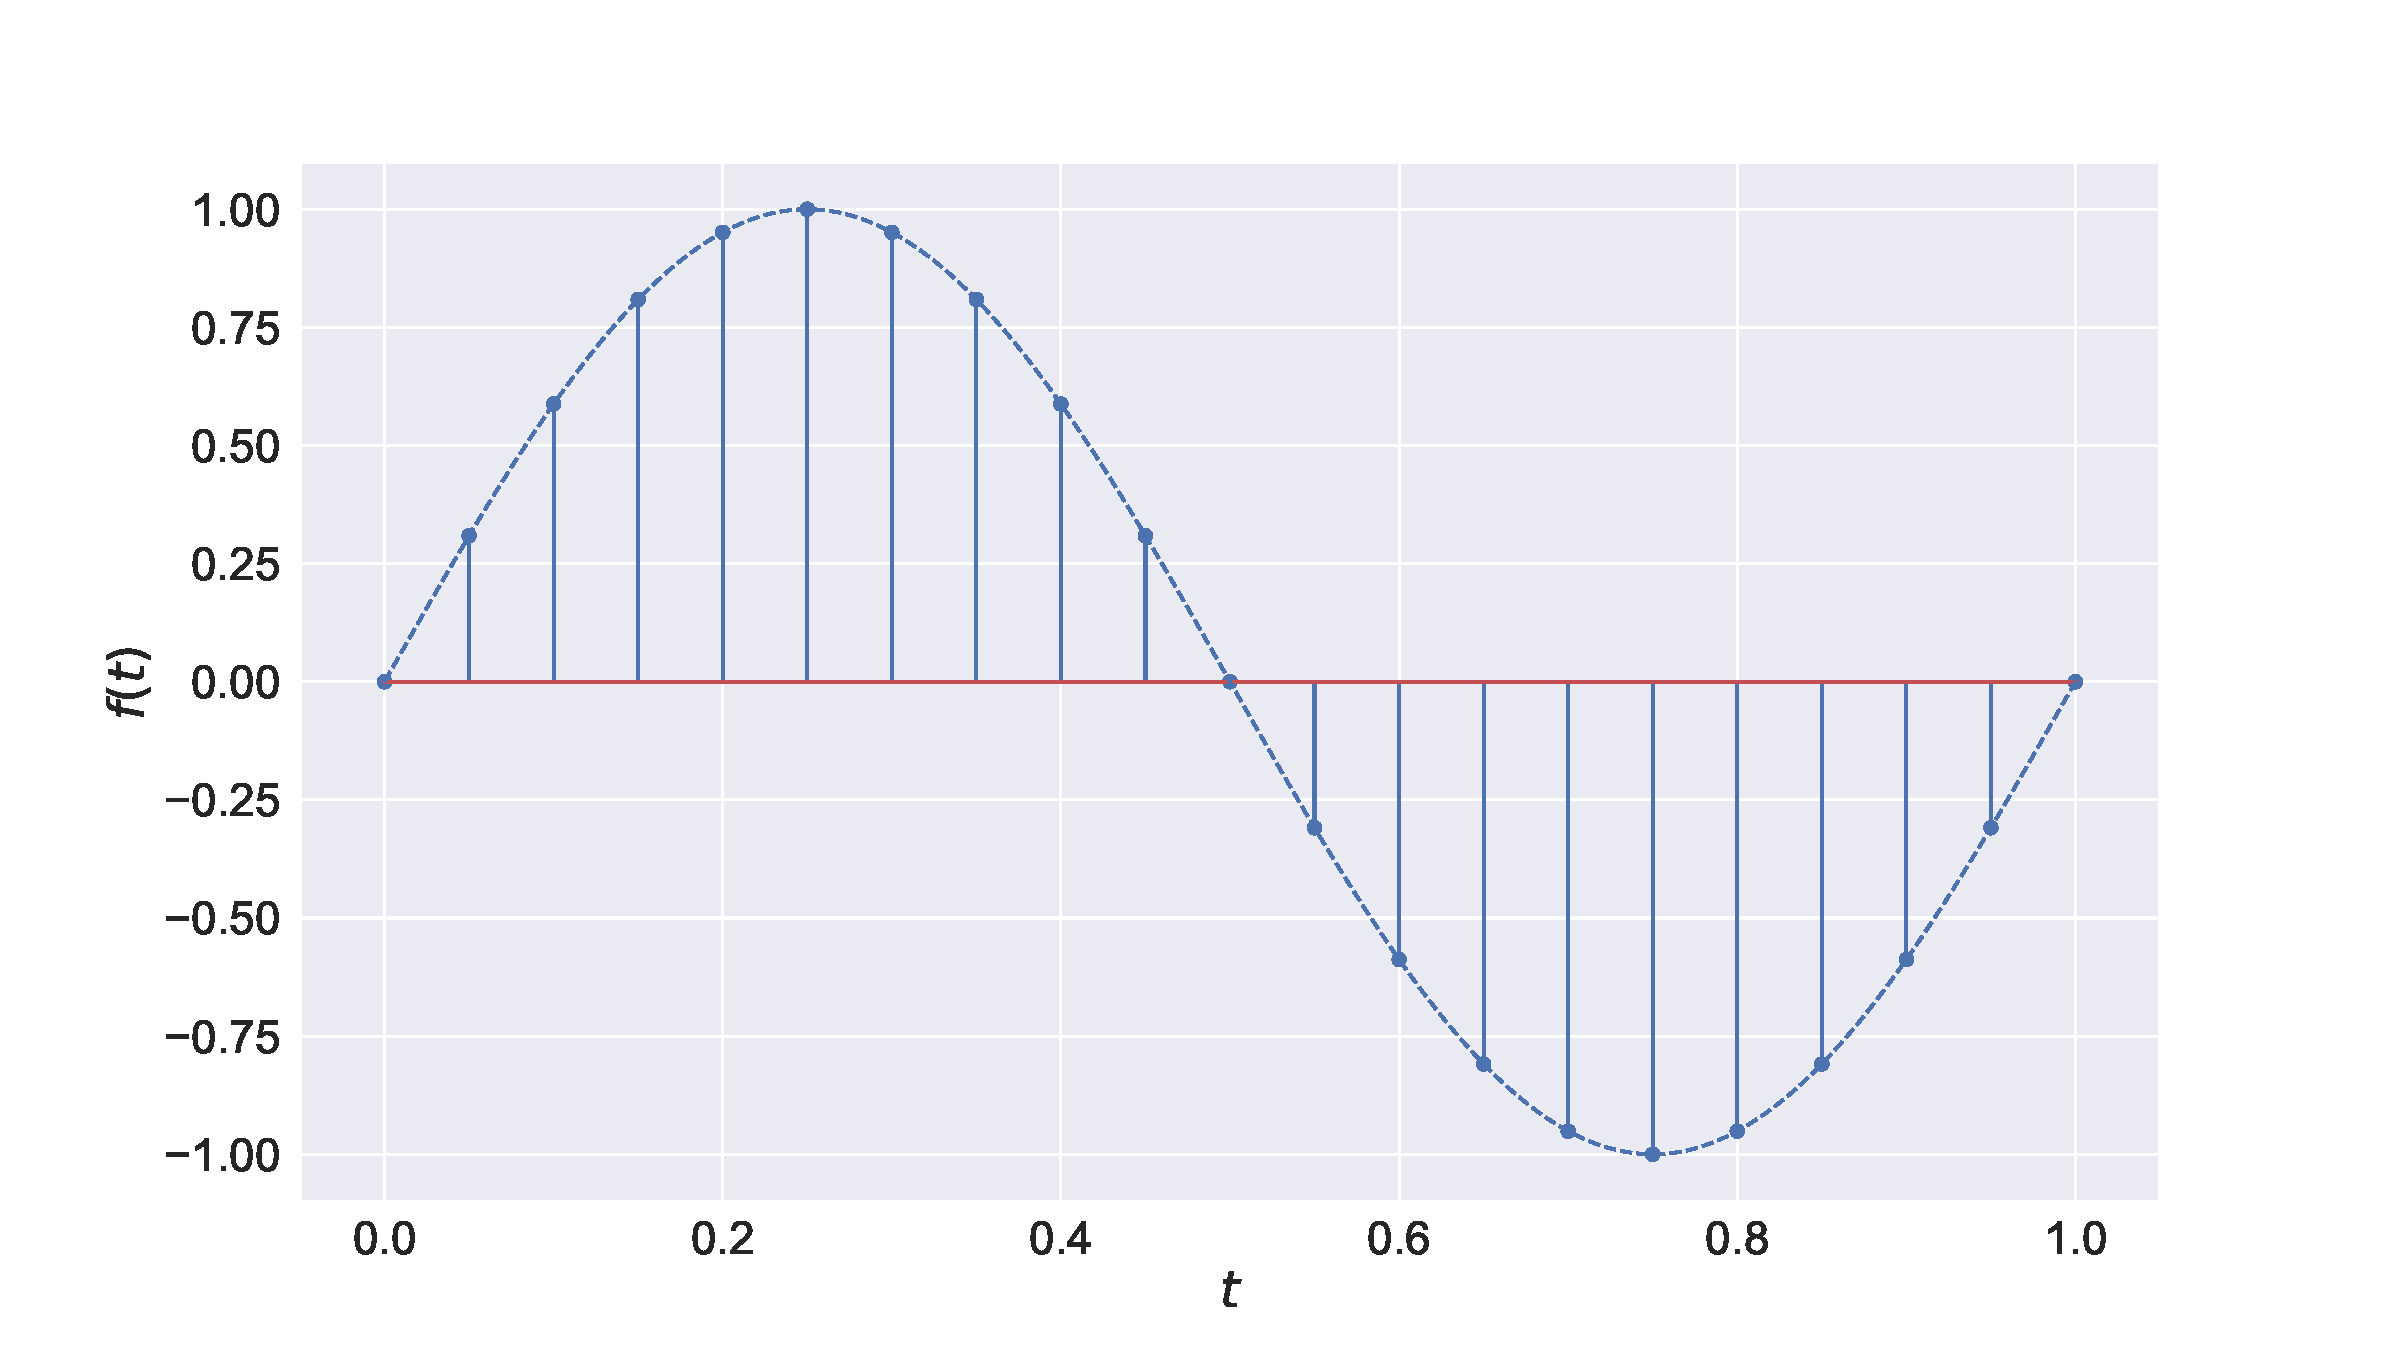
\includegraphics[clip, width=\textwidth]{figure/sin.pdf}
  \caption{離散データの一例}
  \label{fig:digital_sin}
\end{figure}
\fi

この離散データに含まれている周波数成分を算出する手法として離散フーリエ変換が存在する.
離散フーリエ変換とは,式(\ref{eq:dft})で定義される手法であり,
時間領域の離散データ$f(t)$を周波数領域の離散データ$F(\omega)$へ変換することができる.
\begin{align}
  F(\omega) = \sum_{t=0}^{N-1} f(t) e ^ {-j \frac{2 \pi \omega}{N} t} \label{eq:dft}
\end{align}
このとき,式(\ref{eq:dft})における$N$は$f(t)$におけるデータ数である.
式(\ref{eq:dft})では,時間領域の実空間データを複素数空間における三角関数の
総和の形へ変換することにより,時間領域のデータに含まれている周波数成分を算出できる(\autoref{fig:dft}).
\autoref{fig:dft}は\autoref{fig:digital_sin}を離散フーリエ変換したときの周波数領域
データを示している.これより,\autoref{fig:digital_sin}のデータは,1Hz, 6Hz, 10Hzの周波数を
含むことがわかる.

また,周波数領域$F(\omega)$は離散フーリエ逆変換(式(\ref{eq:idft}))
を用いることで時間領域の離散データ$f(t)$へ復元することができる(\autoref{fig:idft}).
\begin{align}
  f(t) = \frac{1}{N}\sum_{\omega=0}^{N-1} F(\omega) e ^ {j \frac{2 \pi t}{N} \omega} \label{eq:idft}
\end{align}
\iffigure
\begin{figure}[h]
  \centering
  \begin{minipage}{.45\hsize}
    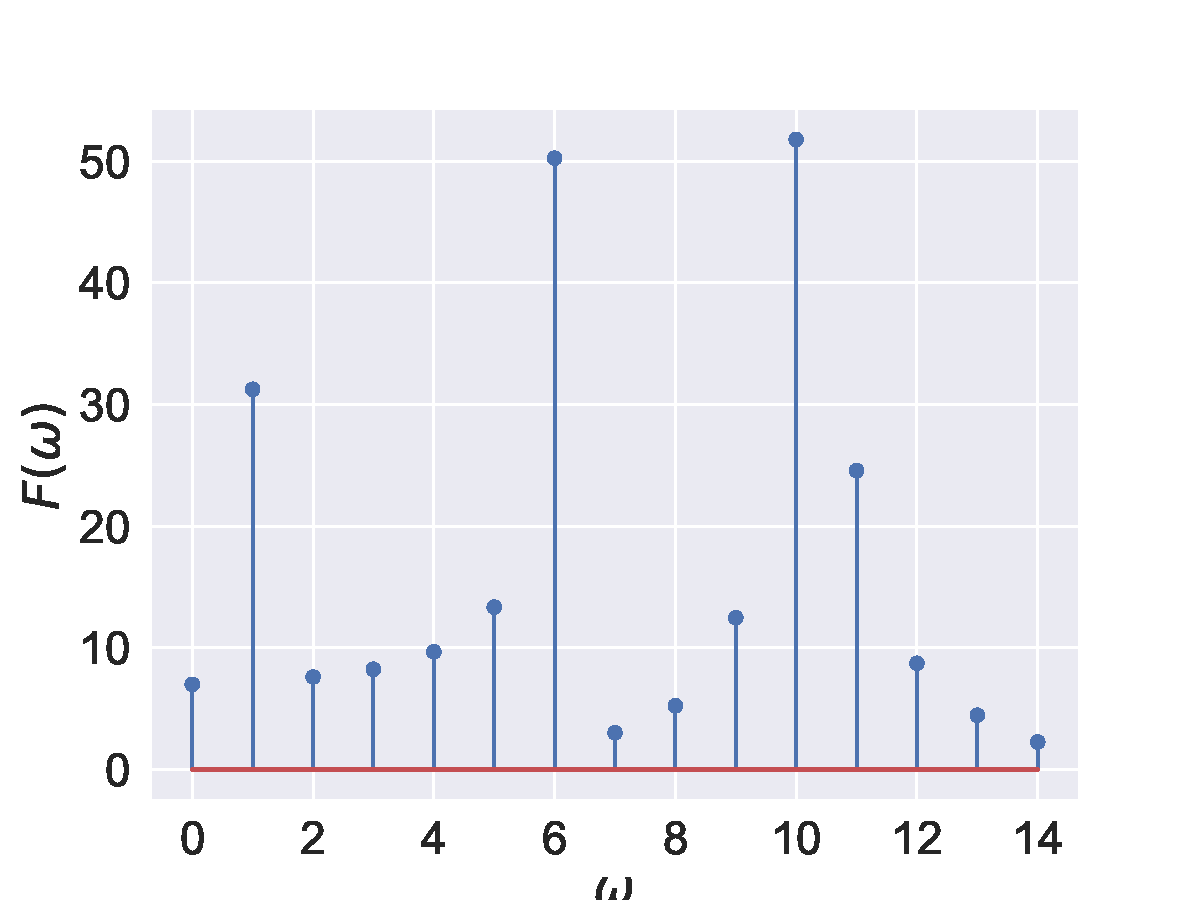
\includegraphics[clip, width=\textwidth]{figure/sin_dft.pdf}
    \caption{\autoref{fig:digital_sin}を式(\ref{eq:dft})を用いて周波数領域の離散データに変換}
    \label{fig:dft}
  \end{minipage}
  \begin{minipage}{.45\hsize}
    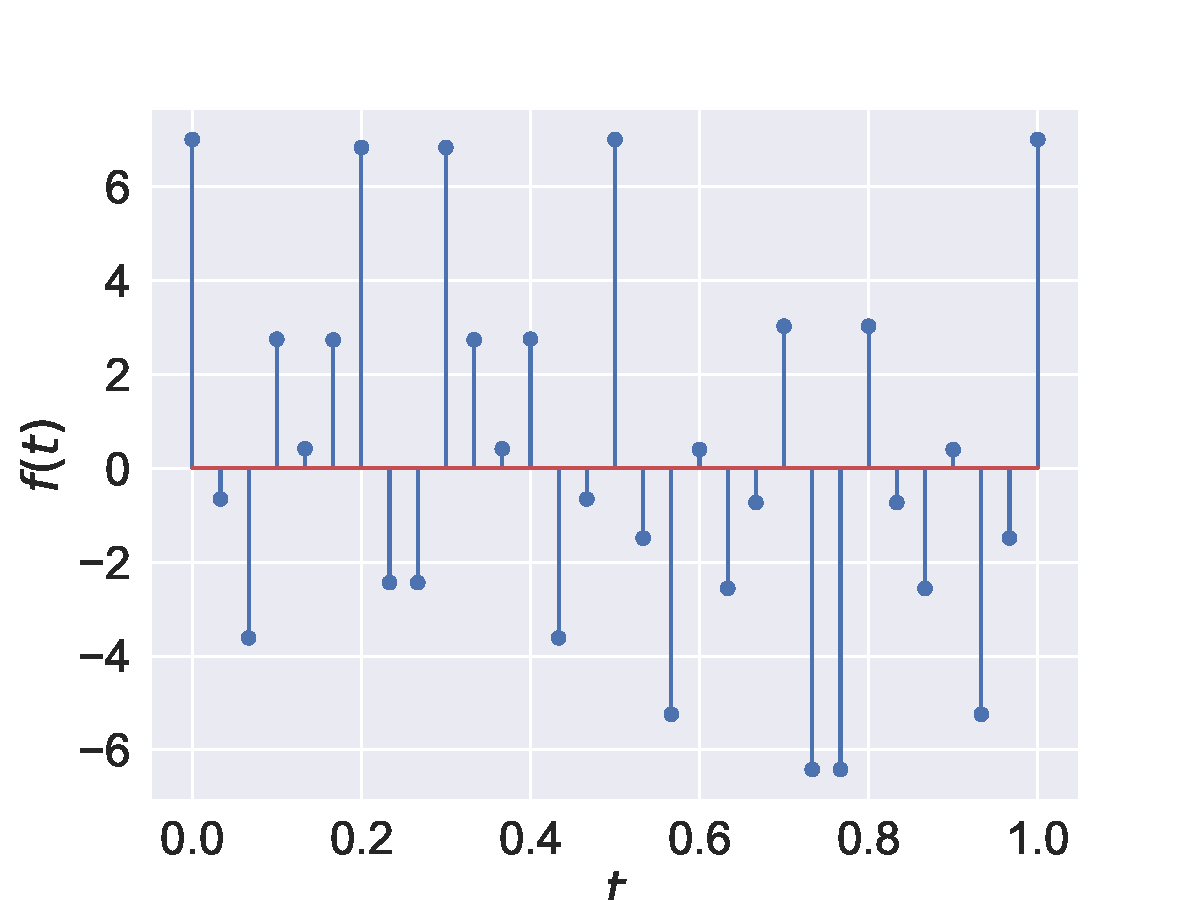
\includegraphics[clip, width=\textwidth]{figure/sin_idft.pdf}
    \caption{\autoref{fig:dft}を式(\ref{eq:idft})を用いて時間領域の離散データに逆変換}
    \label{fig:idft}
  \end{minipage}
\end{figure}
\fi
